% TEX program = xelatex
% compile: xelatex -> biber/bibtex -> xelatex -> xelatex
\documentclass[lang=cn,11pt,a4paper]{elegantpaper}

%%% Title
\title{Laplacian Surface Editing 实验报告}
\author{121090003    Bao Jingzhi}
\institute{CUHK(SZ)}
\date{\zhtoday}

%%% main
\usepackage{array}
\usepackage{wrapfig}
\usepackage{listings}
\usepackage{xcolor}
\usepackage{fontawesome}
\newcommand{\myref}[1]{Eq.\ ref{#1}}
\newcommand{\ccr}[1]{\makecell{{\color{#1}\rule{1cm}{1cm}}}}

\begin{document}

\maketitle

%%% cove
\begin{figure}[ht]
\centering
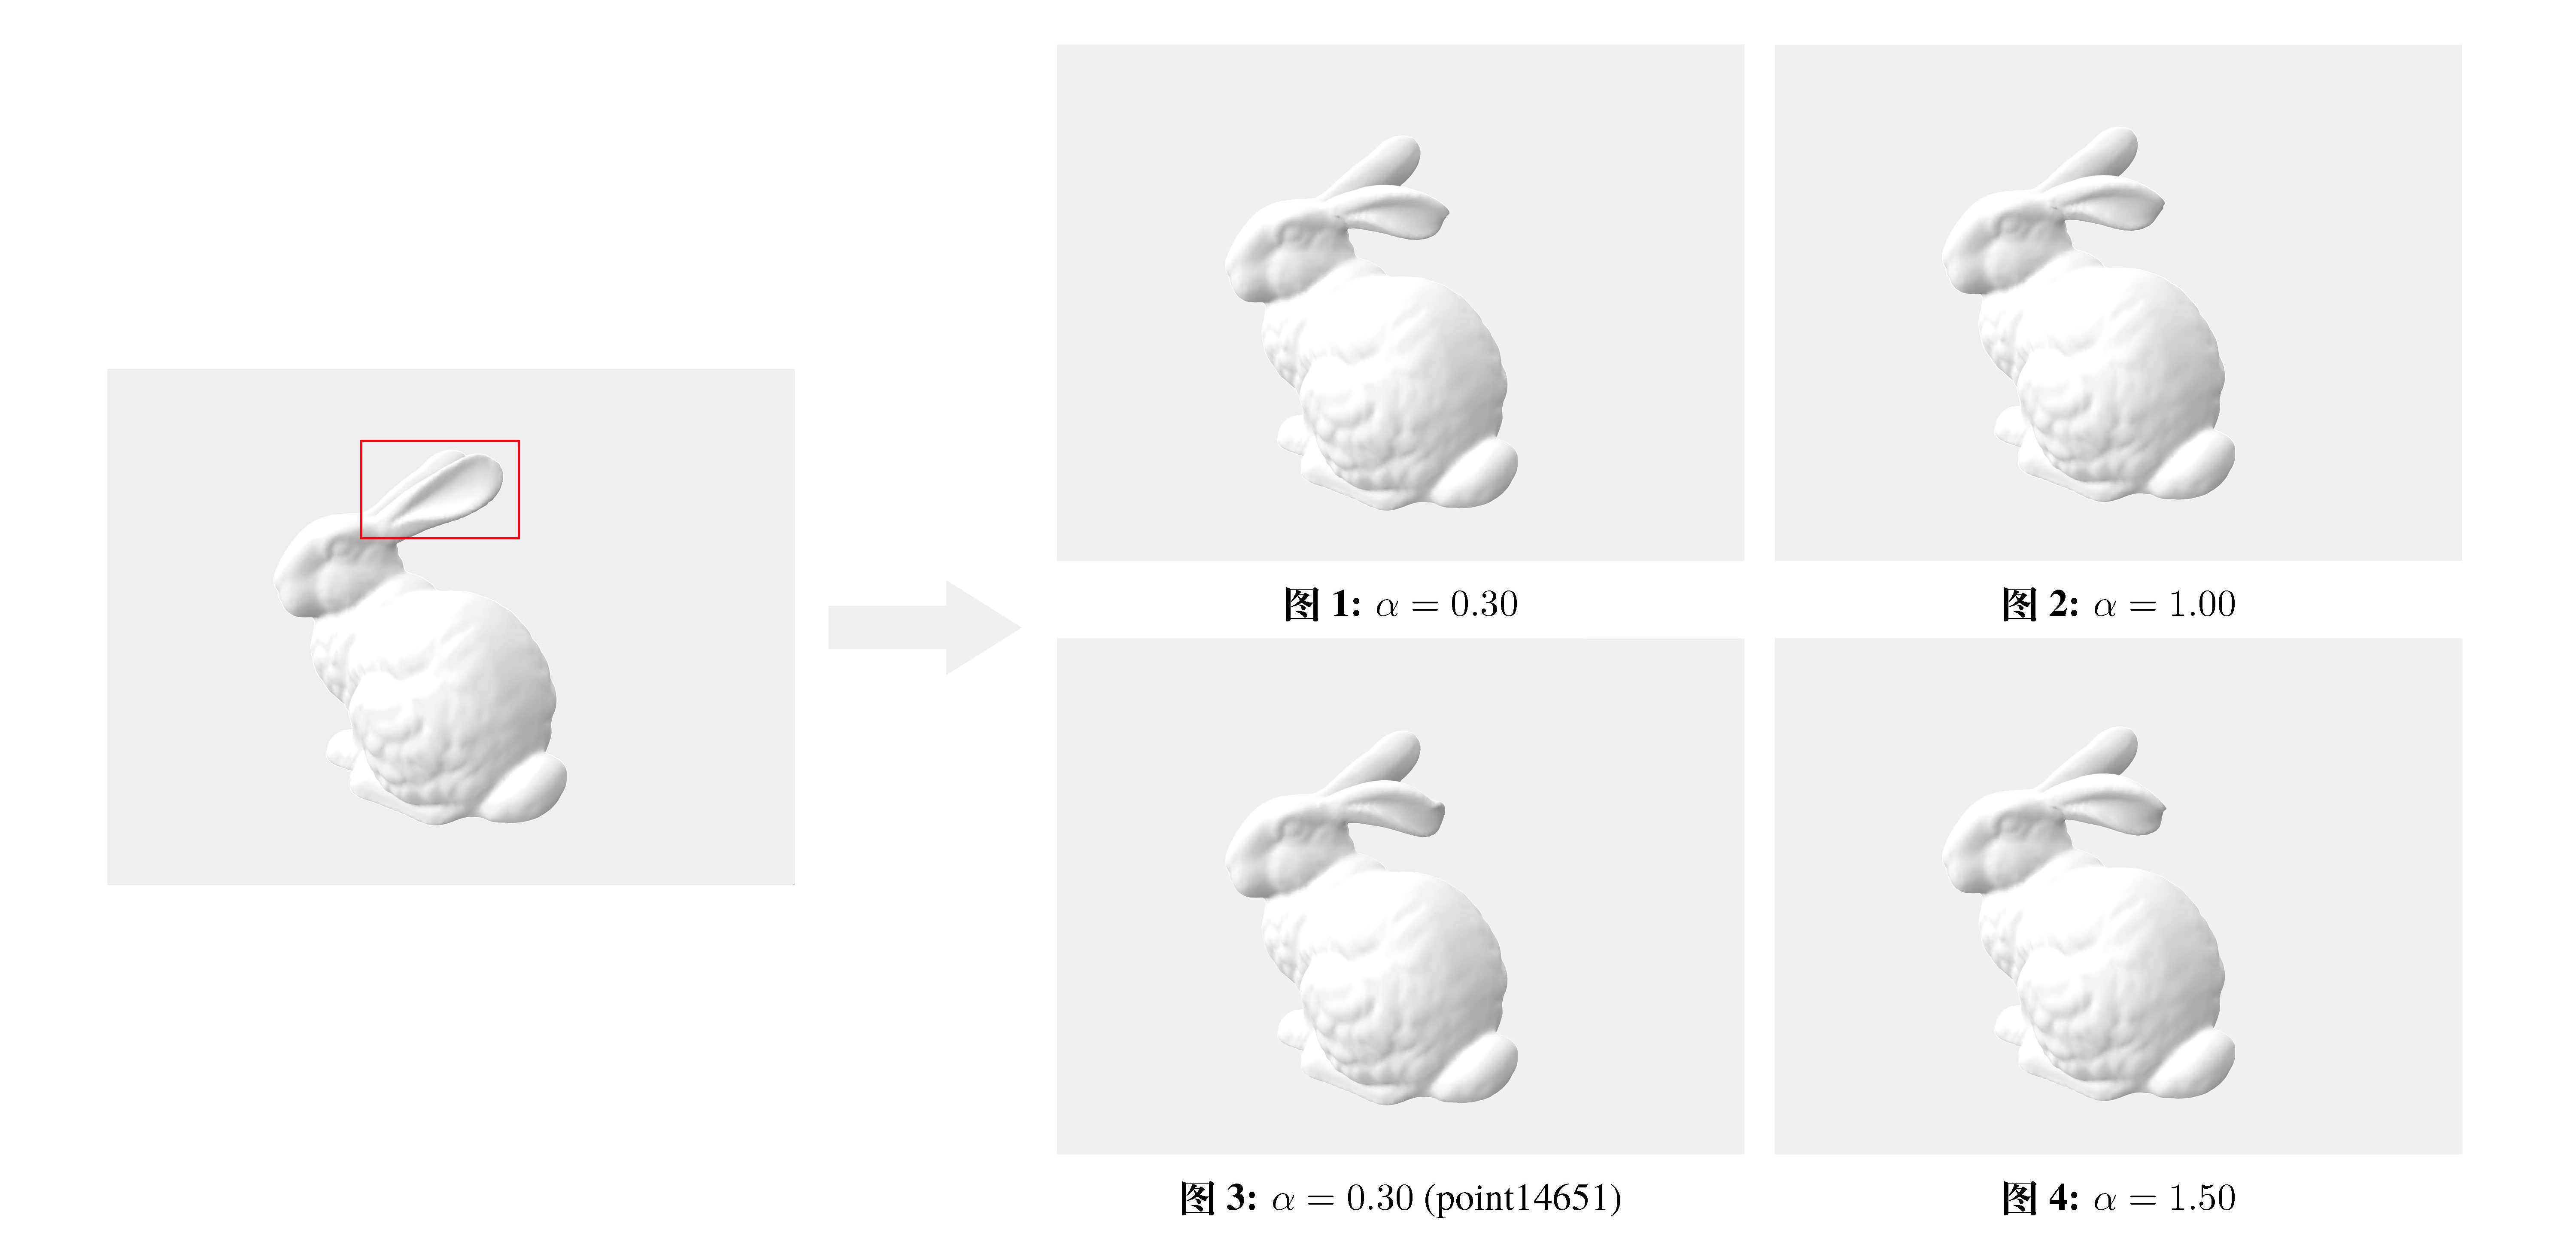
\includegraphics[width=0.999\linewidth]{image/cv3_display.jpg} 
\end{figure}

%%% learning objective
\section{预备知识}
\begin{itemize}
    \item[*] 3D 文件(*.obj, *.mtl, *.ply)的读写和转换
	\item[*] 使用 igraph, NetworkX 等工具进行建图
    \item[*] 利用 Laplacian 算子进行微分坐标与笛卡尔坐标的转换
    \item[*] 带限制凸优化问题的转换
	\item[*] \href{http://www.math.tau.ac.il/~dcor/articles/2004/Laplacian-Surface-Editing.pdf}{Laplacian Surface Editing}\footnote{Source code is available on \faGithubAlt~ \href{https://github.com/ZqlwMatt/CV-project}{GitHub: ZqlwMatt/CV-project}.}
\end{itemize}

\section{开发环境}

\noindent
\textbf{IDE}:Microsoft Visual Studio Code (Universal)\\
\textbf{Python}:3.10.4

\newpage

\section{Laplacian Surface Editing}

\subsection{问题描述}

\begin{figure}[ht]
	\begin{minipage}{0.5\linewidth}
		\centering
		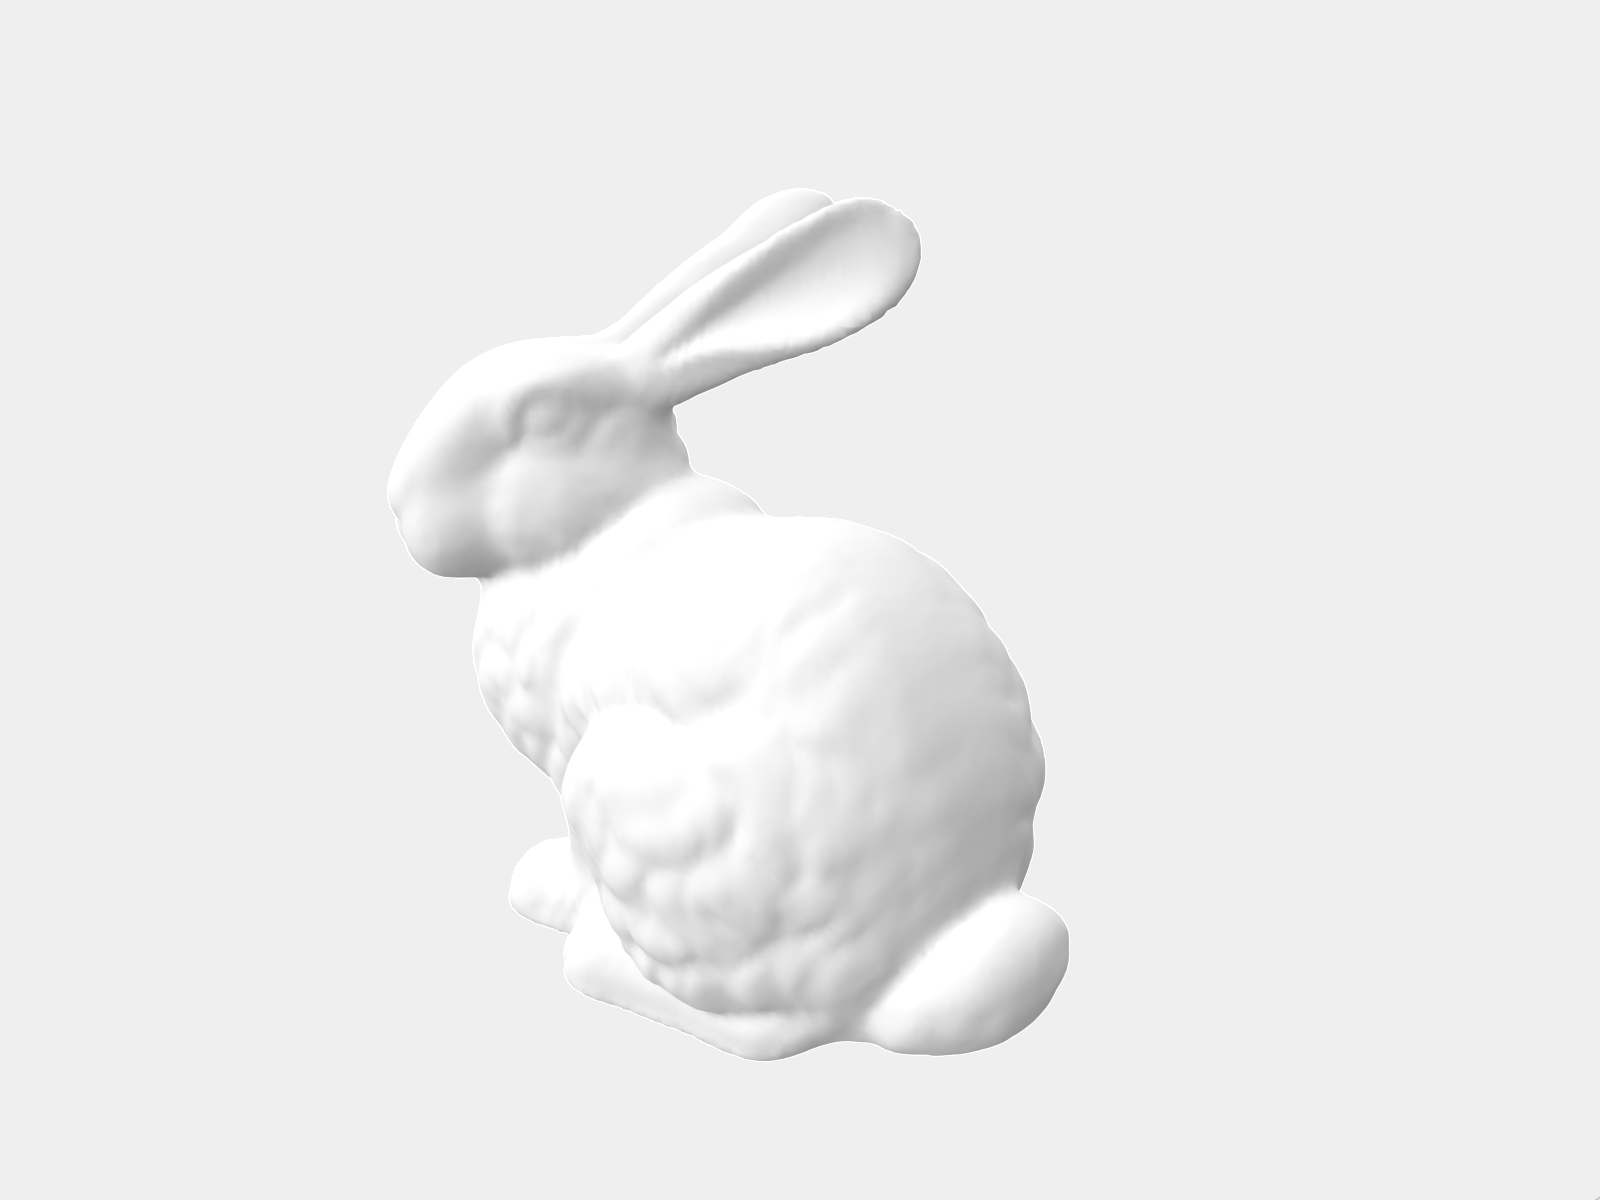
\includegraphics[width=0.85\linewidth]{image/bun_zipper.png}
	\end{minipage}%
	\begin{minipage}{0.5\linewidth}
		\centering
		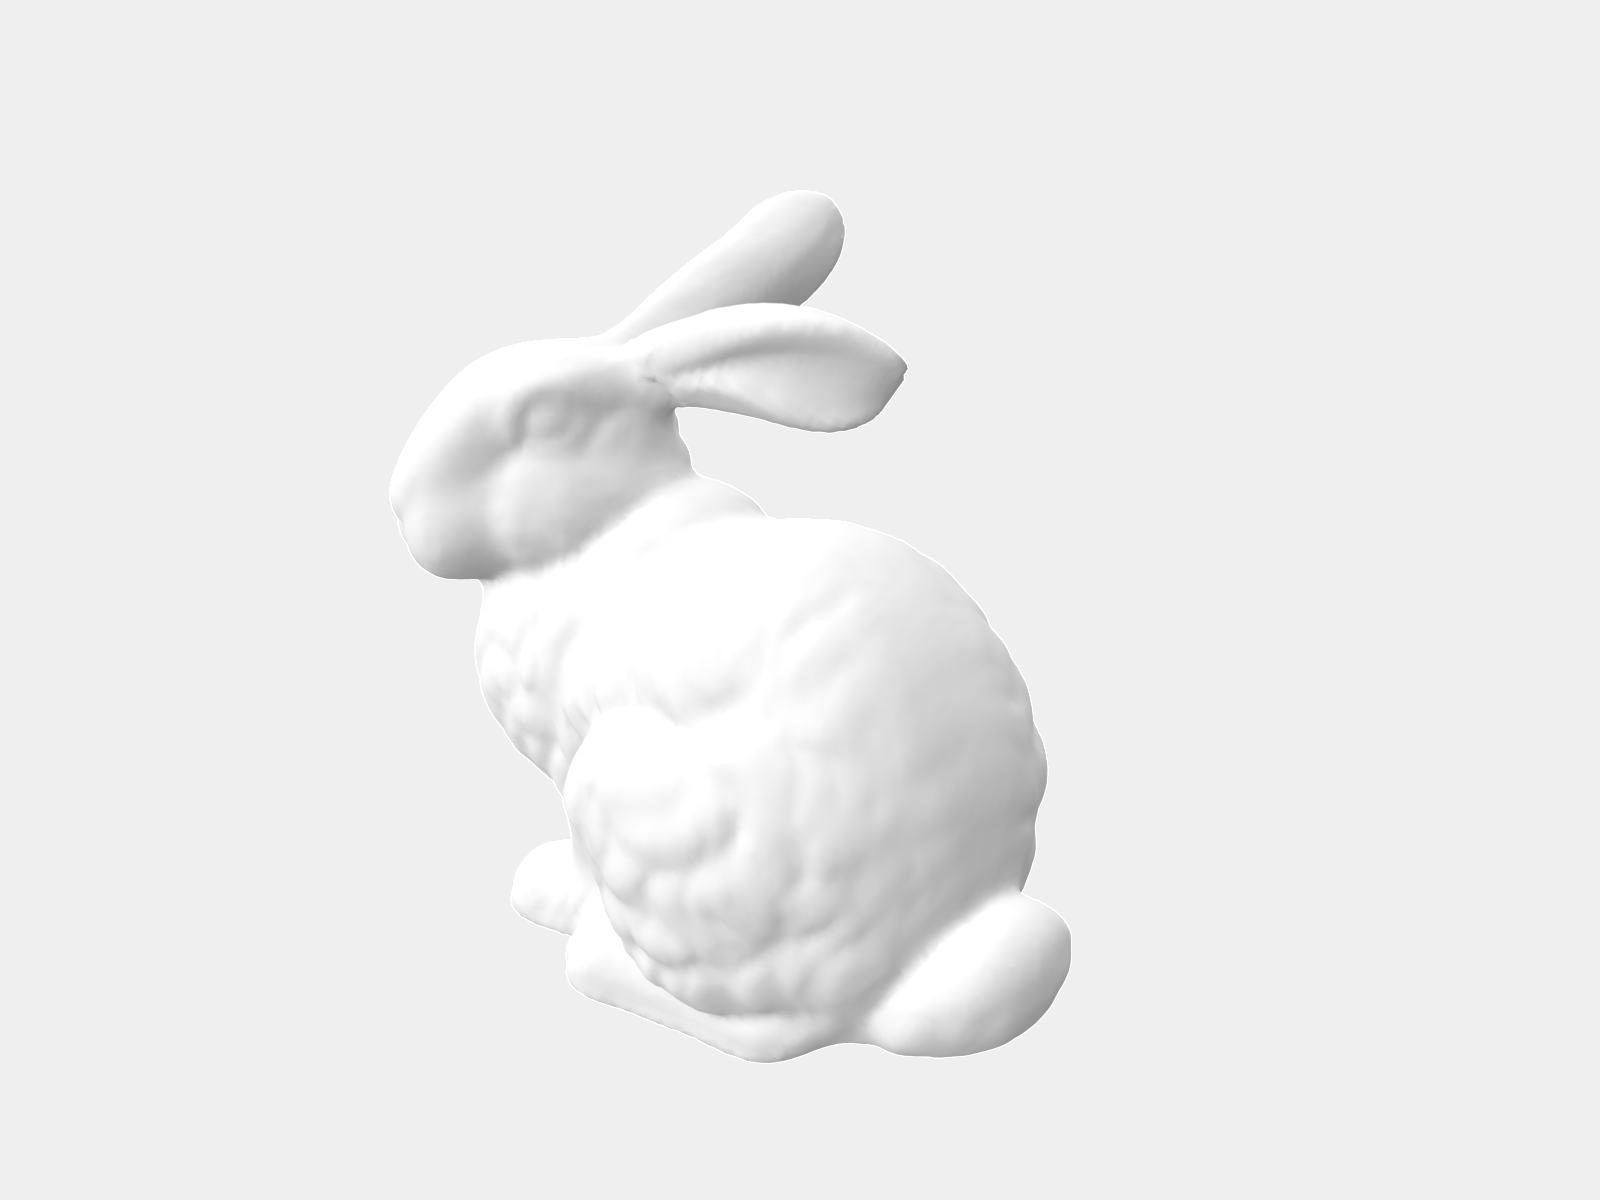
\includegraphics[width=0.85 \linewidth]{image/result_alpha_1.0.png}
	\end{minipage}
\end{figure}

我们需要对指定的3D模型进行局部编辑,要求尽可能地保持模型原有的特征。
示例图片展示了兔子耳朵的弯曲过程。

\subsection{算法描述}

\subsubsection{思路}

对于模型的局部形变操作,顶点的笛卡尔坐标并不重要。这是因为模型的表面特征与{\heiti 微分坐标}(Laplacian coordinates)相关,因此 Laplacian Surface Editing 的思路是保持模型形变前后的微分坐标不变,{\heiti 在不改变面结构(拓扑结构)的条件下}保证模型表面的细节特征。

更具体地,微分坐标有 uniform, weighted least squares 和 shape-preserving [Floater 1995] 三种类型,它们都是笛卡尔坐标的凸结合,在 Laplacian Surface Editing 中都适用,论文选用的是 uniform 类型:

\begin{equation}
    \delta_i = \mathbf{v}_{i}-\frac{1}{d_{i}} \sum_{j \in {N}_{i}} \mathbf{v}_{j}
\end{equation}

依据上式构造 Laplacian 算子 $L = I - D^{-1} A = D^{-1} L_G$ ($L_G$ 为图的 Laplacian Matrix),微分坐标 $\Delta$ 和 $V$ 有转换关系:

\begin{equation}
    \Delta = L V
\end{equation}

设顶点的个数为 $n$,注意到 $\sum\delta_i = 0$,所以 $\text{Rank}(L) = n-1$,因此只要在 $L$ 上扩展一维形变点(handle point)的信息,根据初始模型的 $\delta$ 建立等式 $\delta = L^{\prime} V$,就可以求出形变后的点的坐标 $V$。

值得注意的是,我们需要的是{\heiti 局部区域}经过{\heiti 旋转}得到的结果,上述方程仅支持全局模型重建。论文的重点是下面的优化方法。

\subsubsection{局部编辑}

为实现局部编辑,一个想法是固定模型的部分点,仅对部分点作用 Laplacian 算子。这时 $\delta = L^{\prime} V$ 不一定存在解,问题可以近似转化为最小化函数

\begin{equation}
    E(V^{\prime})=\sum_{i=1}^{n} \| \delta_{i}-L(\mathbf{v}_{i}^{\prime})\|^{2}\ \  \mathrm{with}\ \  \mathbf{v}_{j}^{\prime}=\mathbf{u}_{j}, \ j \in\{m, \ldots, n\}, m<n.
\end{equation}

带限制的最优化问题可以转化为

\begin{equation}
    E(V^{\prime})=\sum_{i=1}^{n} \| \delta_{i}-L(\mathbf{v}_{i}^{\prime})\|^{2}+ \alpha \sum_{i=m}^{n}\| \mathbf{v}_{i}^{\prime}-\mathbf{u}_{i} \|^{2}.
\end{equation}

其中 $\alpha$ 为常数,论文给出的函数默认 $\alpha = 1$。

\subsubsection{模型仿射变换}

微分坐标只保证了模型在平移和全局旋转下的特征,模型 (a) 经过局部变换后得到的模型 (b), (c),$\delta_i$ 不再表示红色点和黄色点形成的向量,但我们认为下图的 (a), (b), (c) 具有相同的细节,因为 (b), (c) 是 (a) 分别经过旋转和缩放得到的。

\begin{figure}[ht]
\centering
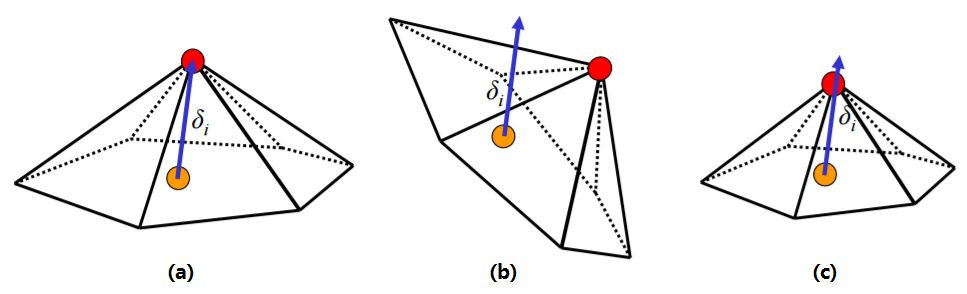
\includegraphics[width=0.9\linewidth]{image/laplacian_rotation.jpeg} 
\end{figure}

为了给 $\delta_i$ 同时提供旋转和缩放的变换,我们可以引入仿射变换矩阵:

\begin{equation}
    T_{i}=\left(\begin{array}{cccc}
s & -h_{3} & h_{2} & t_{x} \\
h_{3} & s & -h_{1} & t_{y} \\
-h_{2} & h_{1} & s & t_{z} \\
0 & 0 & 0 & 1
\end{array}\right).
\end{equation}

那么问题最终转化为:

\begin{equation}
    E(V^{\prime})=\sum_{i=1}^{n} \| T_i\delta_{i}-L(\mathbf{v}_{i}^{\prime})\|^{2}+ \alpha \sum_{i=m}^{n}\| \mathbf{v}_{i}^{\prime}-\mathbf{u}_{i} \|^{2},\label{eq1}
\end{equation}
\begin{equation}
    T_i = \arg\min \left(\left\|T_{i}
    \mathbf{v}_{i}-\mathbf{v}_{i}^{\prime}\right\|^{2}+\sum_{j \in N_{i}}\left\|T_{i} \mathbf{v}_{j}-\mathbf{v}_{j}^{\prime}\right\|^{2}\right).\label{eq2}
\end{equation}

\subsection{方程求解}

求解 Eq.\eqref{eq1} 和 Eq.\eqref{eq2} 是问题的核心,但两者是互相依赖的,无法分别求解。我们显式地写出 $T_i$ 对 $V_i$ 的线性变换,记 $(s_{i}, \vec{h_i}, \vec{t_i})^{T} = (s_{i}, h_{i1}, h_{i2}, h_{i3}, t_{i1}, t_{i2}, t_{i3})^{T}$。我们希望变换后的点和理想点尽可能地相等,即最小化函数

\begin{equation}
\left\|A_{i}\left(s_{i}, \mathbf{h}_{i}, \mathbf{t}_{i}\right)^{T}-\mathbf{b}_{i}\right\|^{2}.
\end{equation}

其中,$A_i$ 为经过调整的邻接矩阵,$\boldsymbol{b}_{i}$ 为最终点的笛卡尔坐标,更具体地

\begin{eqnarray}
A_{i} & = & \left(\begin{array}{ccccccc}
v_{k_{x}} & 0 & v_{k_{z}} & -v_{k_{y}} & 1 & 0 & 0 \\
v_{k_{y}} & -v_{k_{z}} & 0 & v_{k_{x}} & 0 & 1 & 0 \\
v_{k_{z}} & v_{k_{y}} & -v_{k_{x}} & 0 & 0 & 0 & 1 \\
\vdots & & & & & &
\end{array}\right), k \in\{i\} \cup N_{i},
\end{eqnarray}

\begin{eqnarray}
\mathbf{b}_{\mathbf{i}} & = & \left(\begin{array}{c}
v_{k_{x}}^{\prime} \\
v_{k_{y}}^{\prime} \\
v_{k_{z}}^{\prime} \\
\vdots
\end{array}\right), k \in\{i\} \cup N_{i}.
\end{eqnarray}

这个问题的最小二乘解为

\begin{equation}
    (s_{i}, \vec{h_i}, \vec{t_i})^{T} = \left(A_{i}^{T} A_{i}\right)^{-1} A_{i}^{T} \mathbf{b}_{i}\label{eq3}
\end{equation}

注意到 $T_i$ 是一个 $\mathbf{b}_{i}$ 的线性组合,结合 Eq.\eqref{eq3},可以知道 Eq.\eqref{eq1} 的左半部分 $T_i\delta_{i}-L(\mathbf{v}_{i}^{\prime})$ 在 $L^{\prime}$ 中体现为 $\left(A_{i}^{T} A_{i}\right)^{-1} A_{i}^{T} - L_i$。对于 $L^{\prime}$ 的扩展行,则需要根据 Eq.\eqref{eq1} 的右半部分 $\mathbf{v}_{i}^{\prime}-\mathbf{u}_{i}$ ,将 $L^{\prime}$ 的第 $i$ 行赋值为 $\alpha$。至此,$L^{\prime}$ 已经完全构建。

构造矩阵 $B$

\begin{eqnarray}
B & = & \left(\begin{array}{c}
0 \\
0 \\
\vdots \\
0 \\
\alpha \mathbf{u}_{i} \\
\alpha \mathbf{u}_{i+1} \\
\vdots
\end{array}\right)
\end{eqnarray}

Eq.\eqref{eq1} 转化为 $L^{\prime}V^{\prime} = B$。方程的最小二乘解就是我们想要的答案。

注:为方便书写,在提供的代码中 Eq.\eqref{eq1} $L^{\prime}$ 的行按照 $x, y, z$ 的坐标顺序排列,Eq.\eqref{eq2} 按照上文所述的坐标 ${v}_{i} ( x_i, y_i, z_i )$ 顺序排列。

\section{程序实现}

\subsection{提取局部模型}

\begin{figure}[ht]
\centering
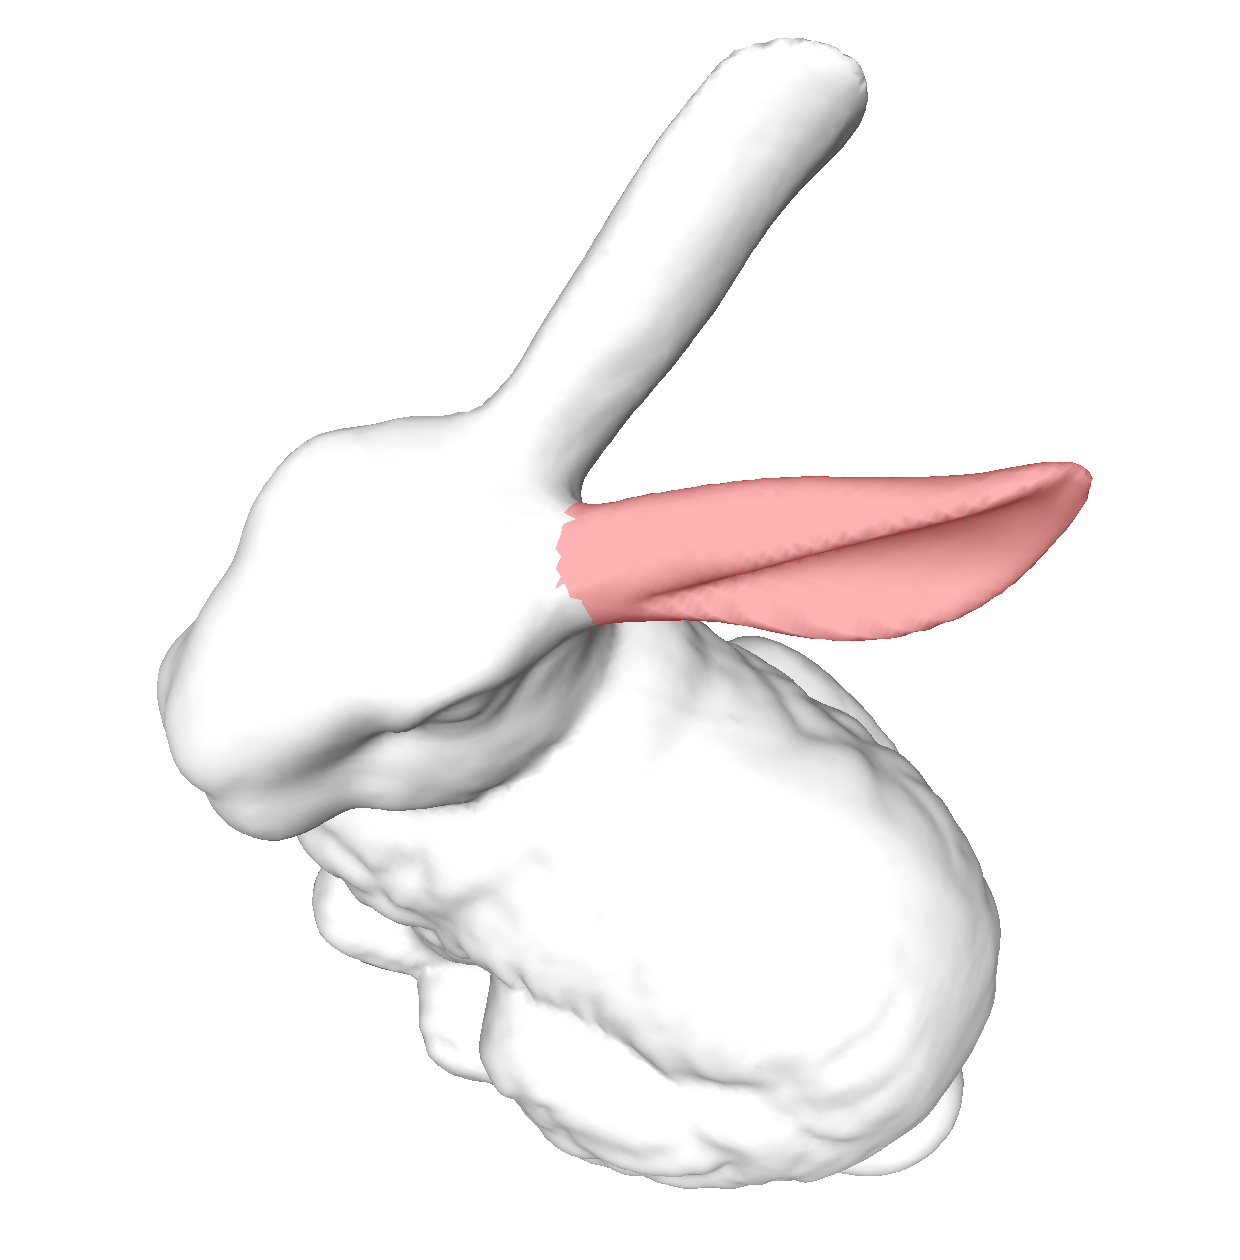
\includegraphics[width=0.33\linewidth]{image/selected_model.png} 
\end{figure}

Laplacian Surface Editing 需要对模型进行局部编辑,我们需要根据提供的固定点求出局部模型,即单连通区域。

\begin{lstlisting}[language=Python]
def get_subgraph(g, ROI_vertices):
    border = []
    for i in range(len(ROI_vertices)):
        segment = g.get_shortest_paths(ROI_vertices[i], ROI_vertices[(i+1)%n], output='vpath')[0]
        border += segment[0:-1]
    g1 = g.to_networkx().remove_nodes_from(border)
    return list(nx.node_connected_component(g1, vertex))
\end{lstlisting}

\subsection{Laplacian 算子}

\begin{lstlisting}[language=Python]
D = np.diag(sub_g.degree(list(range(n))))
Lap = np.array(sub_g.laplacian())
L = np.linalg.inv(D).dot(Lap)
Delta = np.dot(L, sub_V)
\end{lstlisting}

\subsection{方程求解}

\begin{lstlisting}[language=Python]
# Ti x delta
Ti_delta = np.array([
      Delta_ix*   si - Delta_iy*hi[2] + Delta_iz*hi[1], # x 的T变换方程
      Delta_ix*hi[2] + Delta_iy*   si - Delta_iz*hi[0], # y 的T变换方程
    - Delta_ix*hi[1] + Delta_iy*hi[0] + Delta_iz*   si  # z 的T变换方程
])
# Least squares method
Lp = scipy.sparse.coo_matrix(Lp)
Vp = scipy.sparse.linalg.lsqr(Lp, b)[0]
\end{lstlisting}

\section{成果展示}

\begin{figure}[ht]
	\centering
	\begin{minipage}{0.45\linewidth}
		\centering
		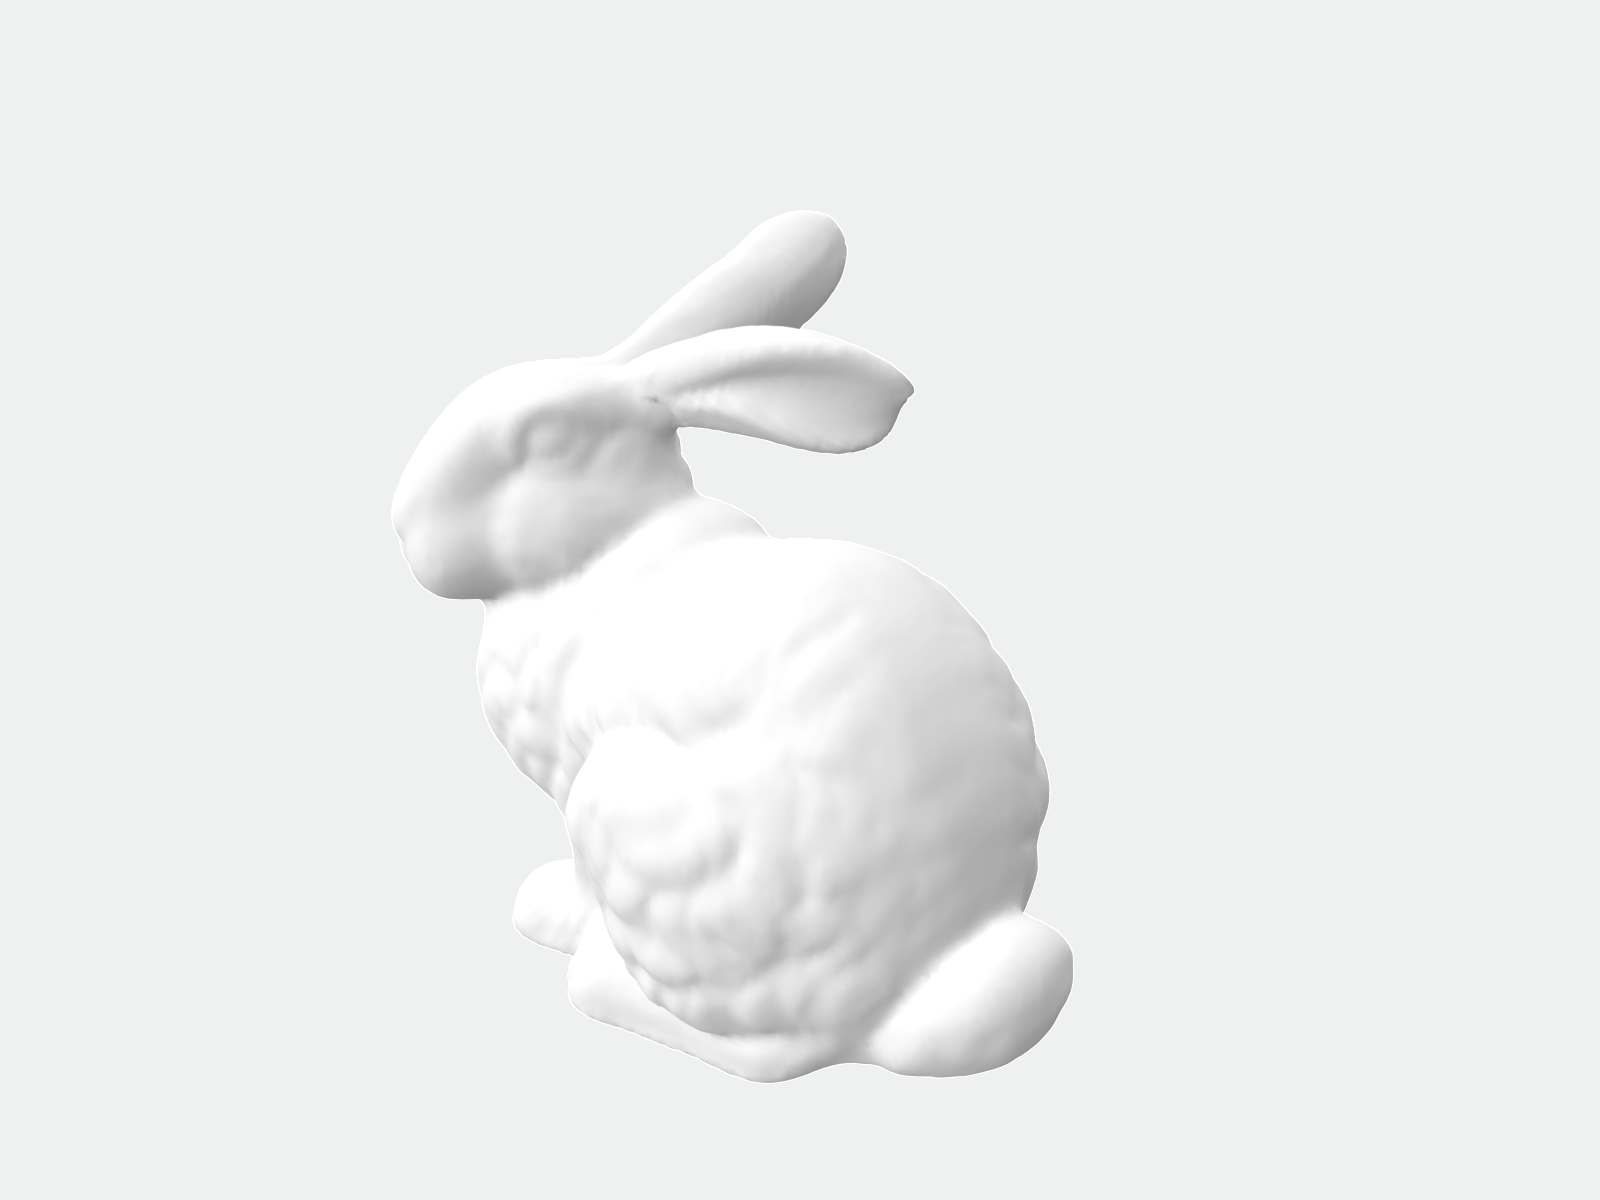
\includegraphics[width=0.97\linewidth]{image/result_alpha_0.3.png}
		\caption{$\alpha = 0.30$}
	\end{minipage}
	\begin{minipage}{0.45\linewidth}
		\centering
		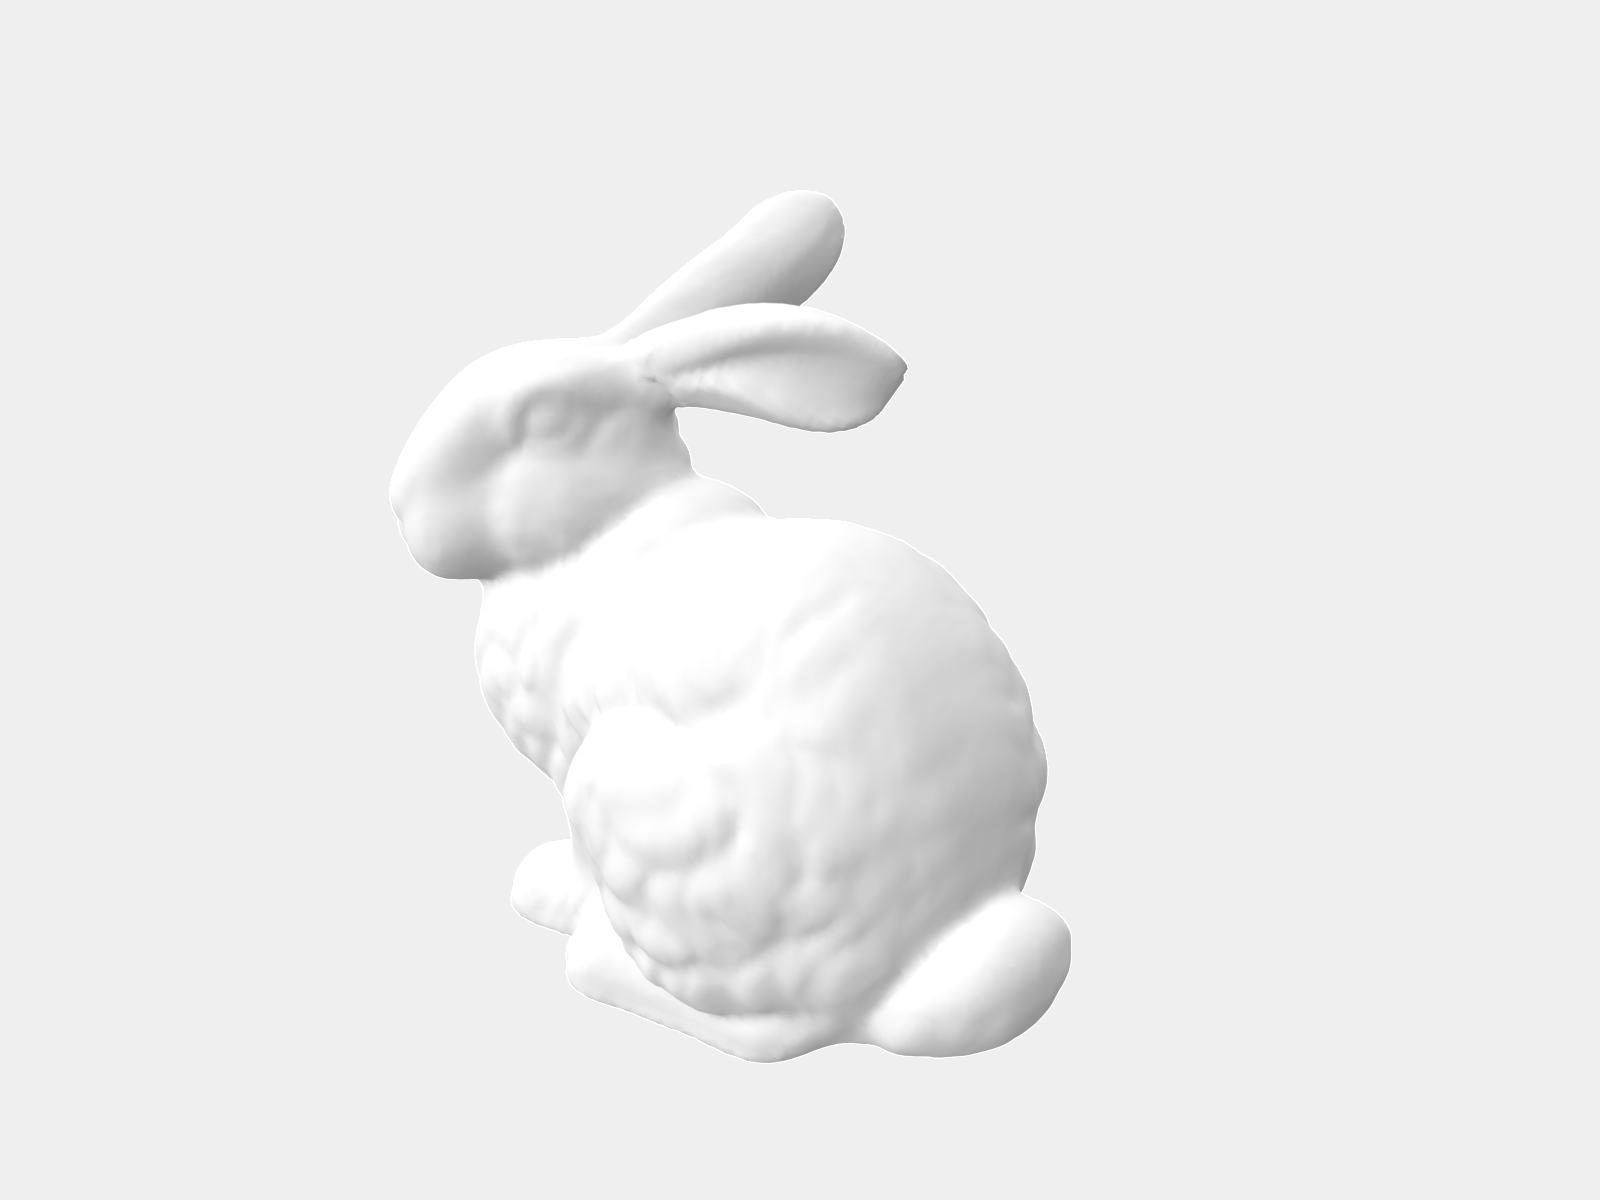
\includegraphics[width=0.97\linewidth]{image/result_alpha_1.0.png}
		\caption{$\alpha = 1.00$}
	\end{minipage}
	%\qquad
	%让图片换行,
	
	\begin{minipage}{0.45\linewidth}
		\centering
		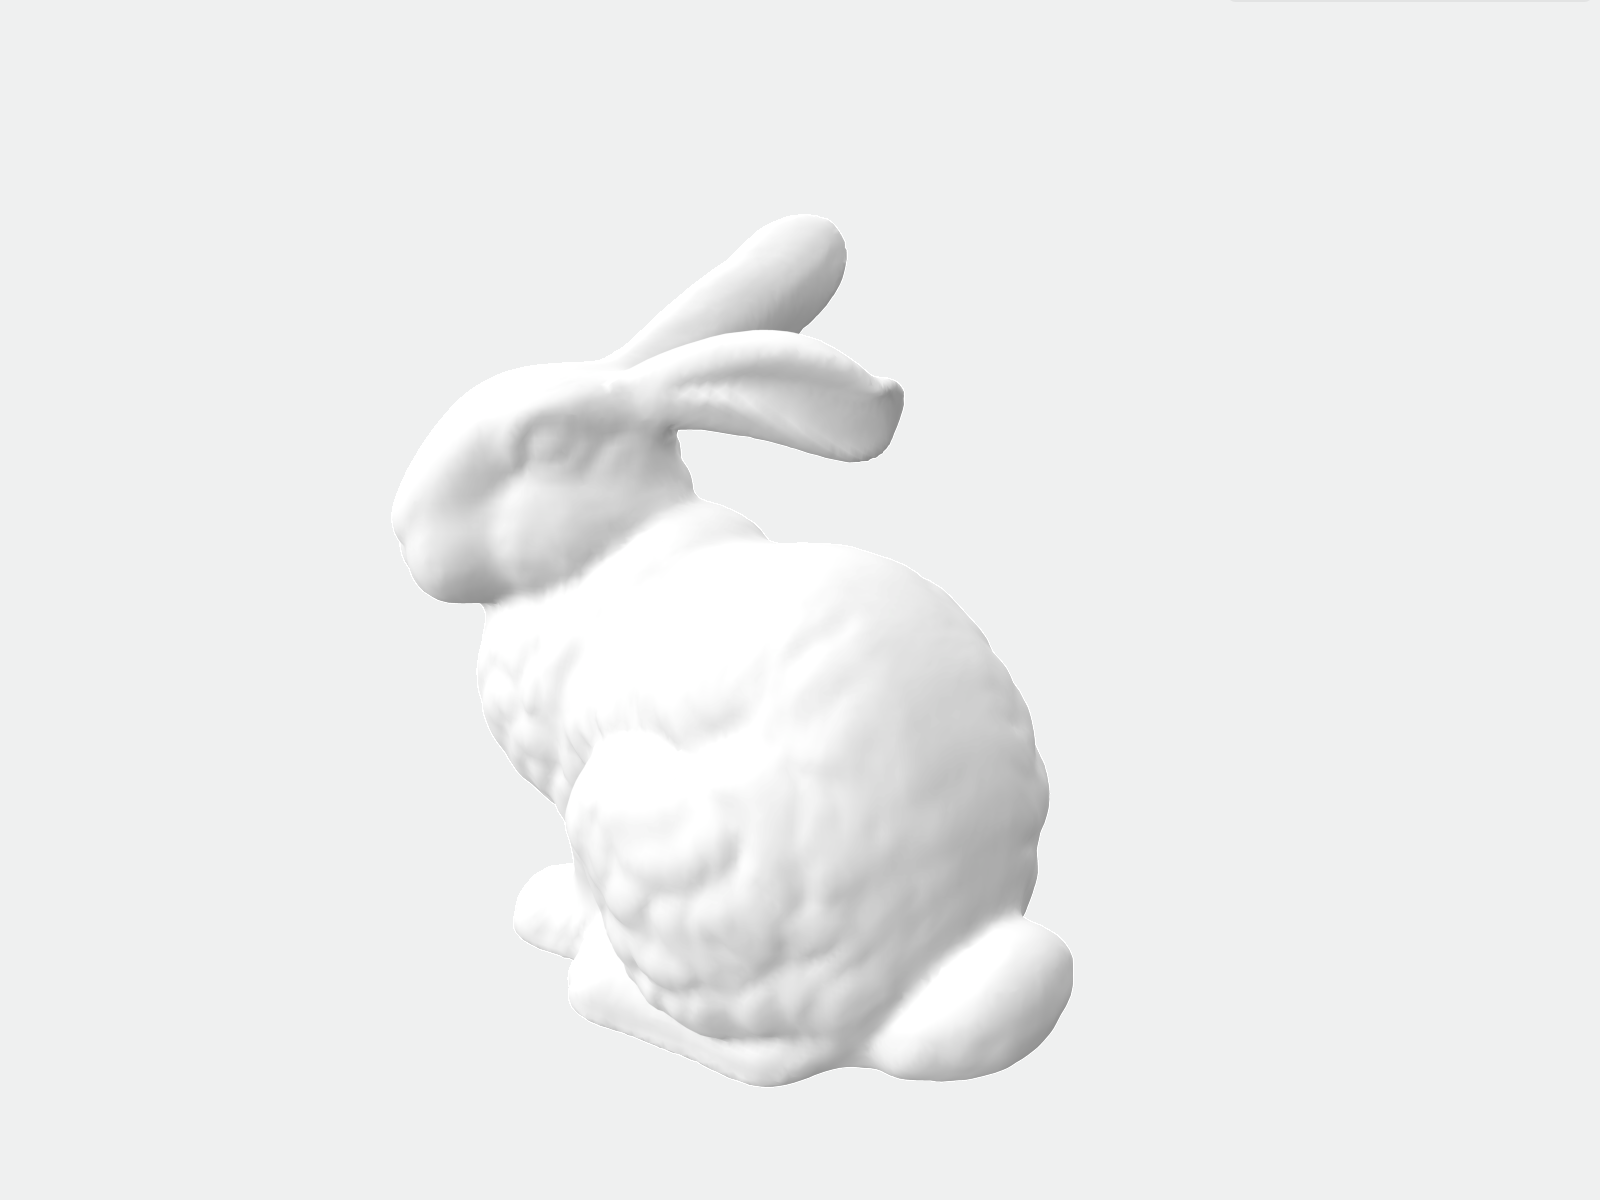
\includegraphics[width=0.97\linewidth]{image/result_point14651_alpha_0.3.png}
		\caption{$\alpha = 0.30$ (point14651)}
	\end{minipage}
	\begin{minipage}{0.45\linewidth}
		\centering
		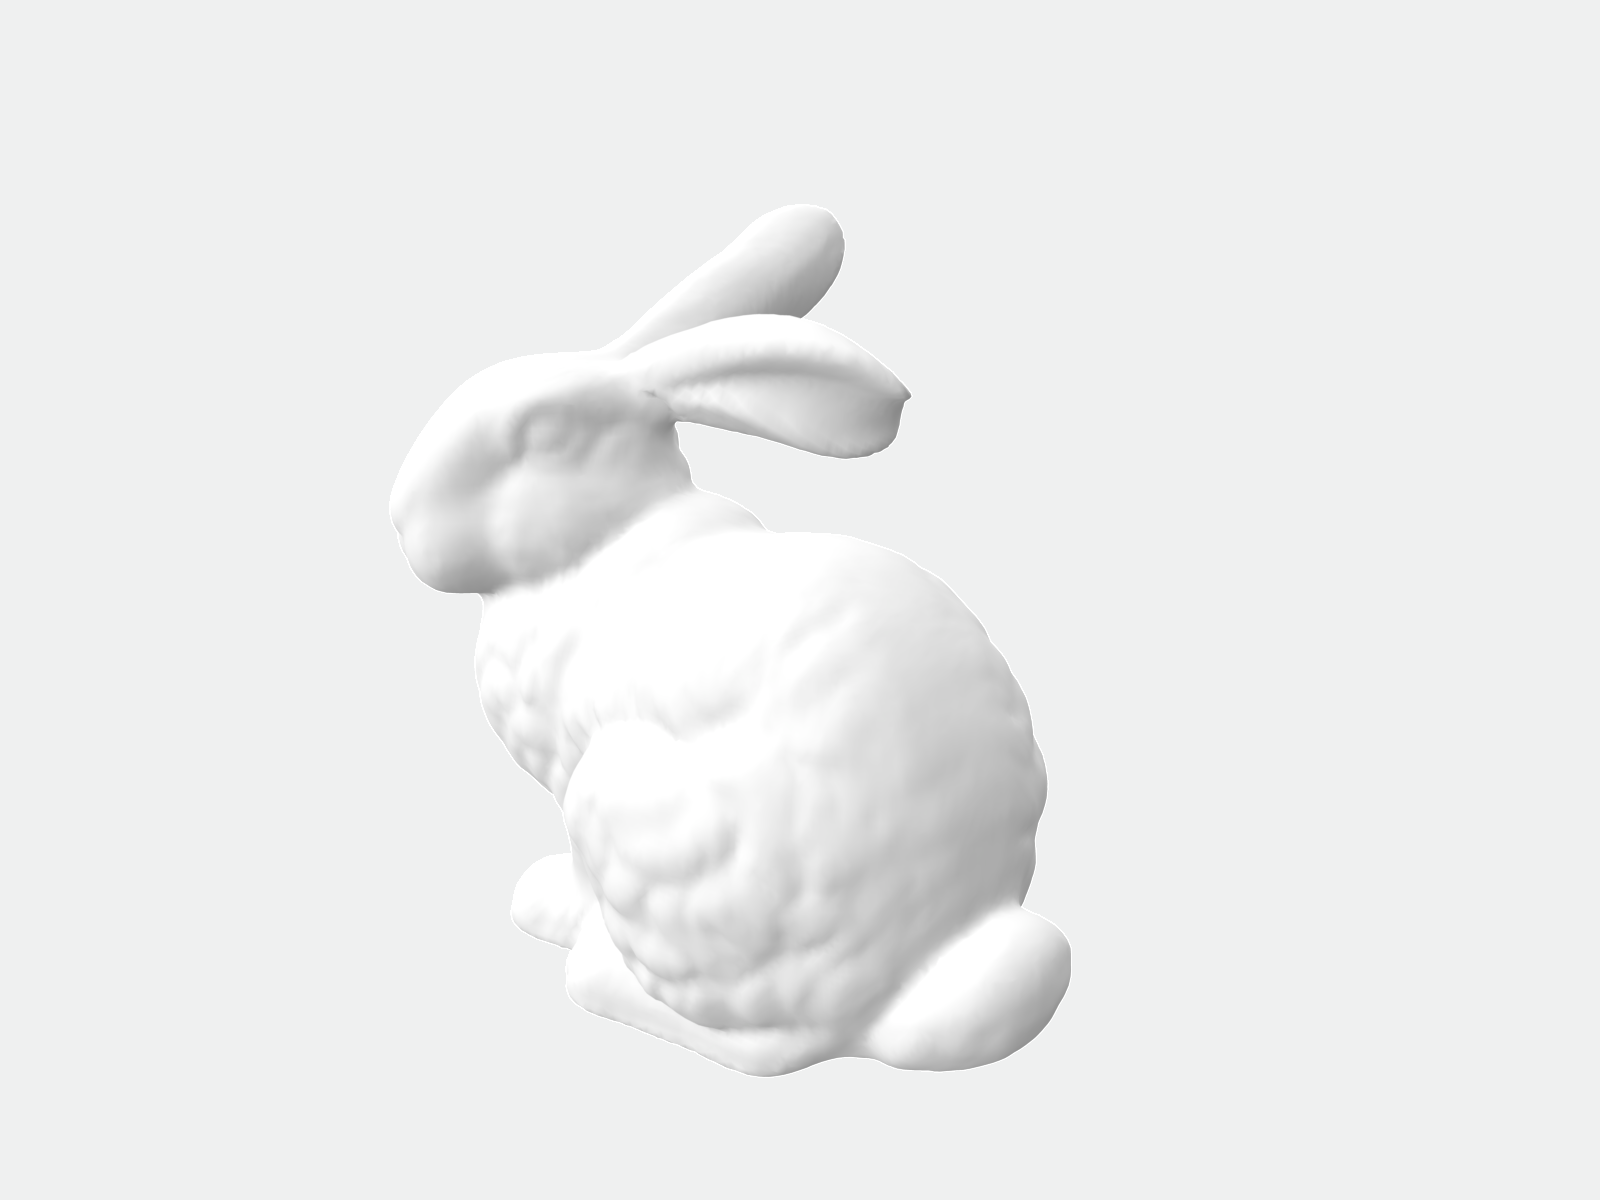
\includegraphics[width=0.97\linewidth]{image/result_alpha_1.5.png}
		\caption{$\alpha = 1.50$}
	\end{minipage}
\end{figure}

\section{算法延伸}

论文中提到了算法的一种应用——涂层迁移,即将一个模型表面的纹理细节映射到另一个模型上。模型表面的涂层可以理解为高频细节 $\xi$ ,具体定义为原模型的微分坐标 $\delta$ 和经过 Laplacian filter 处理后的模型的微分坐标 $\tilde{\delta}$ 的差值

\begin{equation}
    \xi_{i}=\delta_{i}-\tilde{\delta}_{i}
\end{equation}

现在我们得到了模型 1 的局部高频细节 $\xi^{\prime}$,将涂层迁移到模型 2 上只需要将高频细节加到模型 2 的微分坐标 $\Delta$,得到的 $U^{\prime}$ 即为涂层迁移后的点的笛卡尔坐标

\begin{equation}
    U^{\prime}=L^{-1}\left(\Delta+\xi^{\prime}\right)
\end{equation}

但要注意的是,如果我们对不同方向的表面进行涂层迁移,会造成纹理失真,这是因为微分坐标是向量。所以在处理高频细节的时候,我们需要对原模型平滑处理后的表面计算出合适的旋转矩阵。更具体地,点 $\mathbf{v}_{i}$ 的旋转矩阵可以用其邻接点连边在其切平面上的投影向量表示。

\newpage

\begin{figure}[ht]
    \centering
    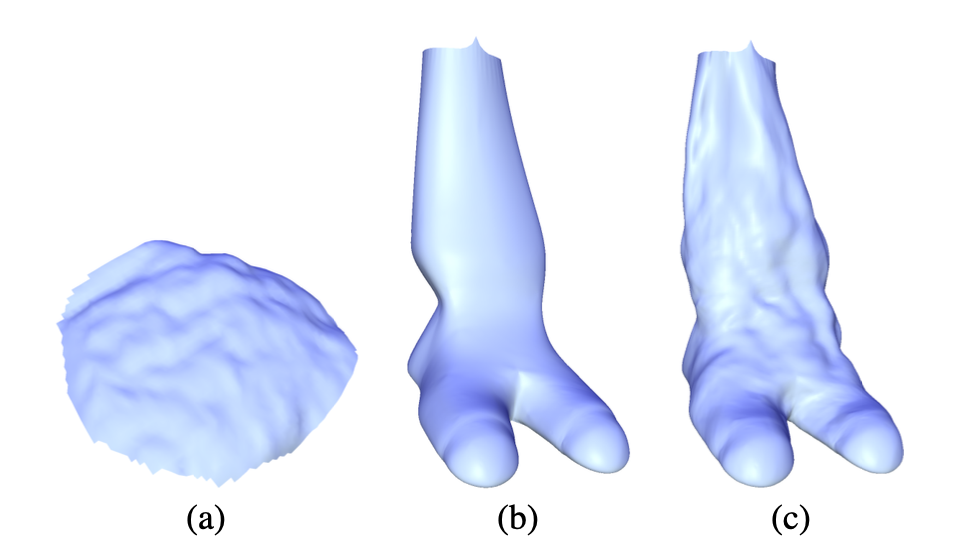
\includegraphics[width=0.5\linewidth]{image/coating_transfer.png}
    \caption{Coating transfer}
\end{figure}

进行局部涂层迁移时还会遇到的一个问题是如何处理模型过度区域的纹理细节。论文采用的方法是混合两者的高频细节,即取两个模型的高频细节的加权均值,这使得模型表面纹理过度更自然。

\begin{equation}
    U^{\prime}=L^{-1}\left(\Delta+\omega_{1}\xi^{\prime}+\omega_{2}\xi_{0}\right), \ w_1+w_2 = 1
\end{equation}

\begin{figure}[ht]
    \centering
    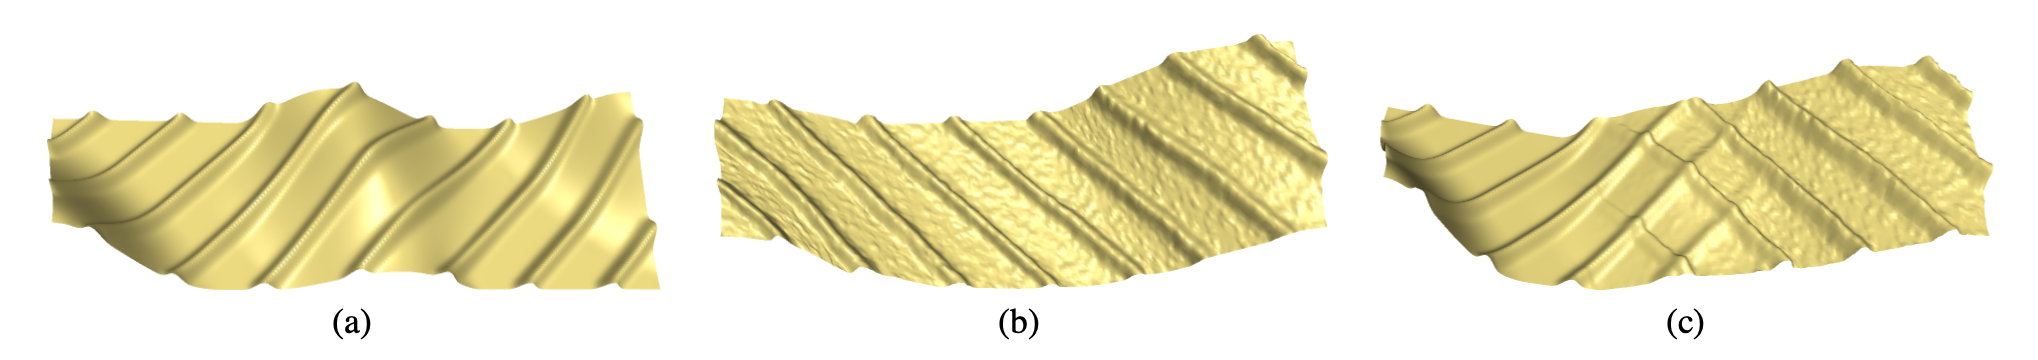
\includegraphics[width=0.95\linewidth]{image/texture_mapping.png}
    \caption{Texture mapping}
\end{figure}


\section{总结}
Laplacian Surface Editing 和 Poisson Image Editing 的思想如出一辙,都是通过保持离散点的 Laplacian Coordinates 进行模型/图像重建,从而保证细节完整。特别地,两者的涂层迁移算法也具有相似性,都是通过取加权和的方式使得过渡区表现自然。

Laplacian Surface Editing 的亮点是构造了旋转矩阵,在对 Laplacian Coordinates 进行方向旋转的同时,使方程仍为线性。

但这种方法的缺点也很明显,在全局重建过程中,如果模型较大,编辑区域顶点产生的矩阵会平方倍增大,内存骤增。方程求解和编辑区域重新参数化的时间也会骤增。


\nocite{*}
\printbibliography[heading=bibintoc, title=\ebibname]

\end{document}
